\documentclass[12pt]{article}
\usepackage[utf8]{inputenc}
\usepackage{graphicx}
\usepackage{booktabs}
\usepackage[margin=1in]{geometry}
\usepackage{amsmath}
\usepackage{amssymb}
\usepackage{enumitem}
\usepackage{caption}
\usepackage{titlesec}
\usepackage{xcolor}
\usepackage{fancyhdr}
\usepackage{microtype}
\usepackage{listings}
\usepackage{framed}
\usepackage{multirow}
\usepackage{float}
\usepackage{makecell}
\usepackage{array}
\usepackage{tabularx}
\usepackage{hyperref}
\usepackage{tikz}
\usetikzlibrary{arrows.meta, positioning, backgrounds, fit, shapes.geometric}
\usepackage{times}  % Times New Roman font

% Code styling for Python
\definecolor{codegreen}{rgb}{0,0.6,0}
\definecolor{codegray}{rgb}{0.5,0.5,0.5}
\definecolor{codepurple}{rgb}{0.58,0,0.82}
\definecolor{backcolour}{rgb}{0.95,0.95,0.92}
\lstdefinestyle{pythonstyle}{
    language=Python,
    basicstyle=\ttfamily\footnotesize,
    keywordstyle=\color{blue}\bfseries,
    commentstyle=\color{codegreen},
    stringstyle=\color{codepurple},
    showstringspaces=false,
    numbers=left,
    numberstyle=\tiny\color{codegray},
    frame=single,
    breaklines=true,
    captionpos=b,
}
\lstset{style=pythonstyle}

% Geometry Setup with sufficient headheight for fancyhdr
\geometry{a4paper, margin=1in, headheight=15pt}

% Title Formatting with section numbering
\titleformat{\section}{\normalfont\Large\bfseries\color{black}}{\thesection}{1em}{}
\titleformat{\subsection}{\normalfont\large\bfseries\color{black}}{\thesubsection}{1em}{}
\titleformat{\subsubsection}{\normalfont\normalsize\bfseries\color{black}}{\thesubsubsection}{1em}{}

% Command for first page border
\newcommand{\firstpageborder}{
    \begin{tikzpicture}[remember picture, overlay]
        \draw[line width=2.5pt, black] 
            ([xshift=15mm, yshift=-10mm]current page.north west) 
            rectangle 
            ([xshift=-15mm, yshift=10mm]current page.south east);
    \end{tikzpicture}
}

\begin{document}

% First page (Cover Page)
\thispagestyle{empty}
\firstpageborder

\begin{center}
    \vspace*{-0.5em}
    {\bfseries\large VIETNAM NATIONAL UNIVERSITY, HO CHI MINH CITY}\\[0.3em]
    {\bfseries\large HO CHI MINH CITY UNIVERSITY OF TECHNOLOGY}\\[0.3em]
    {\bfseries\normalsize FACULTY OF COMPUTER SCIENCE AND ENGINEERING}\\[1.5em]
    
\includegraphics[width=0.22\textwidth]{hcmut.png}
    \vspace{1.8em}

    {\Large\textbf{EMBEDDED SYSTEMS (CO3053)}}\\[0.5em]
    {\large\textbf{Assignment 1: Embedded System Development Process}}\\[0.8em]
    \rule{0.88\textwidth}{0.8pt}\\[0.8em]
    {\LARGE\textbf{Greenhouse Micro-Climate}}\\[0.3em]
    {\LARGE\textbf{Monitoring System}}\\[0.6em]
    {\normalsize\textit{Architectural Solutions, Data Correctness, and Multi-Dimensional Trade-Off Analysis}}\\[0.6em]
    \rule{0.88\textwidth}{0.8pt}
    \vspace{2.2em}

    \begin{minipage}{0.65\textwidth}
        \begin{flushleft}
            \textbf{Instructor:} Dr. Pham Hoang Anh \\
            \textbf{Students:} \\
            \hspace*{1em} Le Thanh Binh - 2352118 \\
            \hspace*{1em} Pham Hong Minh Tu - 2353293 \\
            \hspace*{1em} Pham Minh Nhat - 2352863\\
            \textbf{Class:} CC02
        \end{flushleft}
    \end{minipage}
    \vfill
    {\normalsize HO CHI MINH CITY, September 2026}
    \vspace*{0.5em}
\end{center}

% Clear the header and footer for subsequent pages
\clearpage
\pagestyle{fancy}
\fancyhead[L]{\slshape\footnotesize CO3053 -- Embedded Systems: Assignment 1}
\fancyhead[R]{\slshape\footnotesize Greenhouse Micro-Climate Monitoring}
\renewcommand{\headrulewidth}{0.4pt}
\fancyfoot[C]{}
\fancyfoot[R]{\color{black}Page \thepage}
\pagenumbering{roman}

\begin{abstract}
Micro-climate monitoring is vital for precision agriculture, optimizing photosynthesis, crop yield, and disease prevention while minimizing water and heating energy. This engineering report proposes two comprehensive embedded system architectures to monitor air temperature, relative humidity, and ambient light across an industrial greenhouse measuring $20 \times 50$\,meters ($1{,}000\,\text{m}^2$). The system is evaluated under three critical criteria: \textbf{Communication Infrastructure}, \textbf{Data Correctness}, and \textbf{Real-Time Data Analysis for Anomaly Alerting}. 
\textbf{Design 1} implements a low-power Wireless Sensor Network (WSN) using the LoRaWAN Sub-GHz physical layer in a star-of-stars topology, emphasizing flexibility, rapid deployment, and battery efficiency. 
\textbf{Design 2} utilizes an industrial-grade wired multi-drop bus based on the TIA/EIA-485 (RS-485) physical standard running Modbus RTU, maximizing deterministic polling, zero electromagnetic susceptibility, and centralized power delivery. 
A rigorous multi-dimensional trade-off analysis is presented, evaluating capital expenditure (CAPEX), operational maintenance (OPEX), reliability, latency, and fault containment to provide actionable engineering recommendations.
\end{abstract}

\vspace{0.8cm}
\tableofcontents
\newpage

\pagenumbering{arabic}
\setcounter{page}{1}

% =========================================================================
\section{Introduction and Problem Formulation}
% =========================================================================

\subsection{Greenhouse Operational Environment \texorpdfstring{($20 \times 50$\,m)}{(20x50m)}}
Protected horticulture in an industrial greenhouse measuring $20 \times 50$\,meters ($1{,}000\,\text{m}^2$, with ridge heights typically ranging from $4$ to $6$\,m) presents a hostile and dynamic operating environment for electronic monitoring systems. High humidity cycles (up to $95\%$ non-condensing or condensing during misting cycles), chemical vapors from fertilizers and pest sprays, temperature variations ranging from $15^\circ\text{C}$ to over $45^\circ\text{C}$, and high water-content crop foliage create severe operational challenges:
\begin{enumerate}
    \item \textbf{Radio Frequency (RF) Attenuation:} Lush vegetative canopy acts as a dielectric loss medium that absorbs and scatters electromagnetic radiation in the $2.4\,\text{GHz}$ band (Wi-Fi, Zigbee, Bluetooth).
    \item \textbf{Electromagnetic Interference (EMI):} High-power inductive loads, including circulating fans, automated irrigation pumps, and high-intensity artificial grow lights (HPS or LED drivers), generate transient voltage spikes and radio noise.
    \item \textbf{Spatial Thermal and Hygrometric Stratification:} Stagnant air pockets, localized solar radiation hotspots, and air-vent drafts cause substantial micro-climatic gradients across the $50$\,m axis.
\end{enumerate}

\subsection{Monitored Micro-Climate Parameters}
Optimal greenhouse management requires continuous, synchronized acquisition of three key physical variables:
\begin{itemize}
    \item \textbf{Air Temperature ($T$):} Affects plant transpiration, metabolic enzymes, and floral development. Operating range: $0^\circ\text{C}$ to $60^\circ\text{C}$ with required accuracy $\pm 0.3^\circ\text{C}$.
    \item \textbf{Relative Humidity ($RH$):} Essential for calculating Vapor Pressure Deficit (VPD). Excessive humidity triggers fungal pathogeneity, while very low humidity causes stomatal closure. Operating range: $10\%$ to $100\%$ with accuracy $\pm 2\%$.
    \item \textbf{Ambient Light Intensity / Illuminance ($L$):} Measures Photosynthetically Active Radiation (PAR, $400 - 700\,\text{nm}$) to regulate dynamic shading nets and supplementary lighting. Dynamic range: $0$ to $120{,}000\,\text{lux}$.
\end{itemize}

\subsection{Evaluation Criteria}
As prescribed in the engineering assignment, each proposed architecture must address:
\begin{enumerate}
    \item \textbf{Communication Infrastructure:} Physical topology, network protocol stack, physical transmission media, frequency bands, modulation schemes, and power distribution mechanisms.
    \item \textbf{Data Correctness:} Signal conditioning, transmission error detection and correction (EDC), sensor calibration, physical protection (IP rating), and digital filtering against spurious transient spikes.
    \item \textbf{Data Analysis for Alerting:} Architectural partitioning of intelligence (Edge Computing vs. Cloud Computing), anomaly detection rules, hysteresis thresholding, and automated multi-channel alert delivery (local sirens, SMS, MQTT/Webhooks).
\end{enumerate}

% =========================================================================
\section{Spatial Node Allocation and Hardware Subsystem}
% =========================================================================

\subsection{Spatial Topology and Sensor Distribution Matrix}
To capture micro-climatic gradients across the $1{,}000\,\text{m}^2$ facility without creating spatial blind spots, the greenhouse is divided into a $2 \times 5$ grid of ten monitoring zones ($10 \times 10\,\text{m}$ each). Ten sensor nodes ($N_1$ to $N_{10}$) are suspended at crop canopy height ($1.5\,\text{m}$ above ground). A central gateway/controller is placed at the entrance/service partition ($X=0\,\text{m}, Y=10\,\text{m}$) where primary grid power and telecom infrastructure terminate.

\begin{figure}[H]
\centering
\resizebox{0.92\linewidth}{!}{
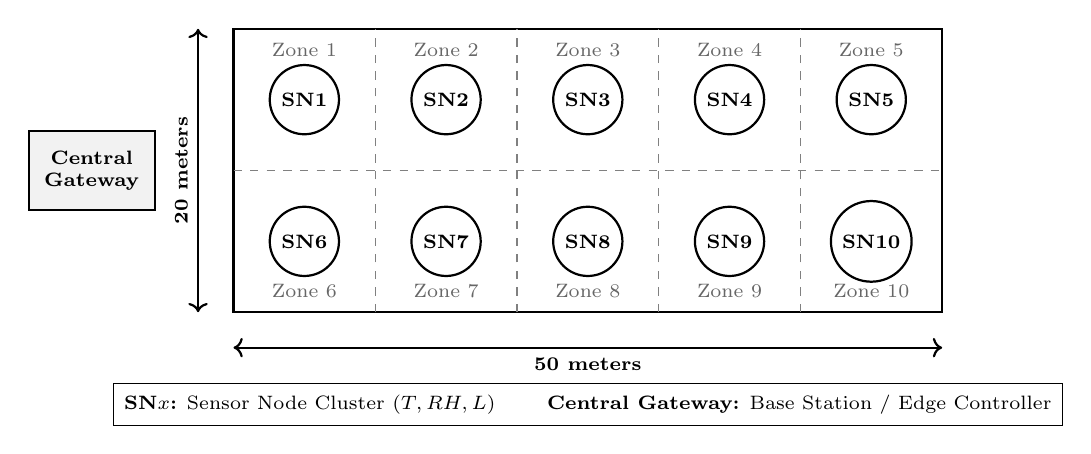
\begin{tikzpicture}[scale=0.18, every node/.style={font=\scriptsize}]
    % Greenhouse border - Draw.io B&W Style
    \draw[thick, fill=white] (0,0) rectangle (50,20);
    \draw[dashed, black!50] (0,10) -- (50,10);
    \foreach \x in {10, 20, 30, 40} {
        \draw[dashed, black!50] (\x,0) -- (\x,20);
    }
    
    % Dimension markers
    \draw[<->, thick, black] (0,-2.5) -- (50,-2.5) node[midway, below] {\textbf{50 meters}};
    \draw[<->, thick, black] (-2.5,0) -- (-2.5,20) node[midway, above, rotate=90] {\textbf{20 meters}};
    
    % Nodes Row 1 (Y = 15m)
    \node[circle, draw=black, fill=white, thick, inner sep=3pt] (N1) at (5,15) {\textbf{SN1}};
    \node[circle, draw=black, fill=white, thick, inner sep=3pt] (N2) at (15,15) {\textbf{SN2}};
    \node[circle, draw=black, fill=white, thick, inner sep=3pt] (N3) at (25,15) {\textbf{SN3}};
    \node[circle, draw=black, fill=white, thick, inner sep=3pt] (N4) at (35,15) {\textbf{SN4}};
    \node[circle, draw=black, fill=white, thick, inner sep=3pt] (N5) at (45,15) {\textbf{SN5}};
    
    % Nodes Row 2 (Y = 5m)
    \node[circle, draw=black, fill=white, thick, inner sep=3pt] (N6) at (5,5) {\textbf{SN6}};
    \node[circle, draw=black, fill=white, thick, inner sep=3pt] (N7) at (15,5) {\textbf{SN7}};
    \node[circle, draw=black, fill=white, thick, inner sep=3pt] (N8) at (25,5) {\textbf{SN8}};
    \node[circle, draw=black, fill=white, thick, inner sep=3pt] (N9) at (35,5) {\textbf{SN9}};
    \node[circle, draw=black, fill=white, thick, inner sep=3pt] (N10) at (45,5) {\textbf{SN10}};
    
    % Gateway at the entrance
    \node[rectangle, draw=black, fill=black!5, thick, minimum width=1.6cm, minimum height=1.0cm, align=center] (GW) at (-10,10) {\textbf{Central}\\\textbf{Gateway}};
    
    % Zone labels
    \node[black!60] at (5,18.5) {Zone 1};
    \node[black!60] at (15,18.5) {Zone 2};
    \node[black!60] at (25,18.5) {Zone 3};
    \node[black!60] at (35,18.5) {Zone 4};
    \node[black!60] at (45,18.5) {Zone 5};
    \node[black!60] at (5,1.5) {Zone 6};
    \node[black!60] at (15,1.5) {Zone 7};
    \node[black!60] at (25,1.5) {Zone 8};
    \node[black!60] at (35,1.5) {Zone 9};
    \node[black!60] at (45,1.5) {Zone 10};
    
    % Legend
    \node[draw=black, fill=white, inner sep=4pt] at (25,-6.5) {
        \textbf{SN$x$:} Sensor Node Cluster ($T, RH, L$) \quad\quad 
        \textbf{Central Gateway:} Base Station / Edge Controller
    };
\end{tikzpicture}
}
\caption{Spatial layout and sensor node deployment matrix across the $20 \times 50$\,m greenhouse facility.}
\label{fig:greenhouse_layout}
\end{figure}

\subsection{Sensor Node Hardware Architecture}
Each sensor node cluster integrates precision transducers, signal conditioning, an ultra-low-power microcontroller unit (MCU), power regulation, and a physical communication transceiver, as depicted in Figure~\ref{fig:node_block_diagram}.

\begin{figure}[H]
\centering
\resizebox{\linewidth}{!}{
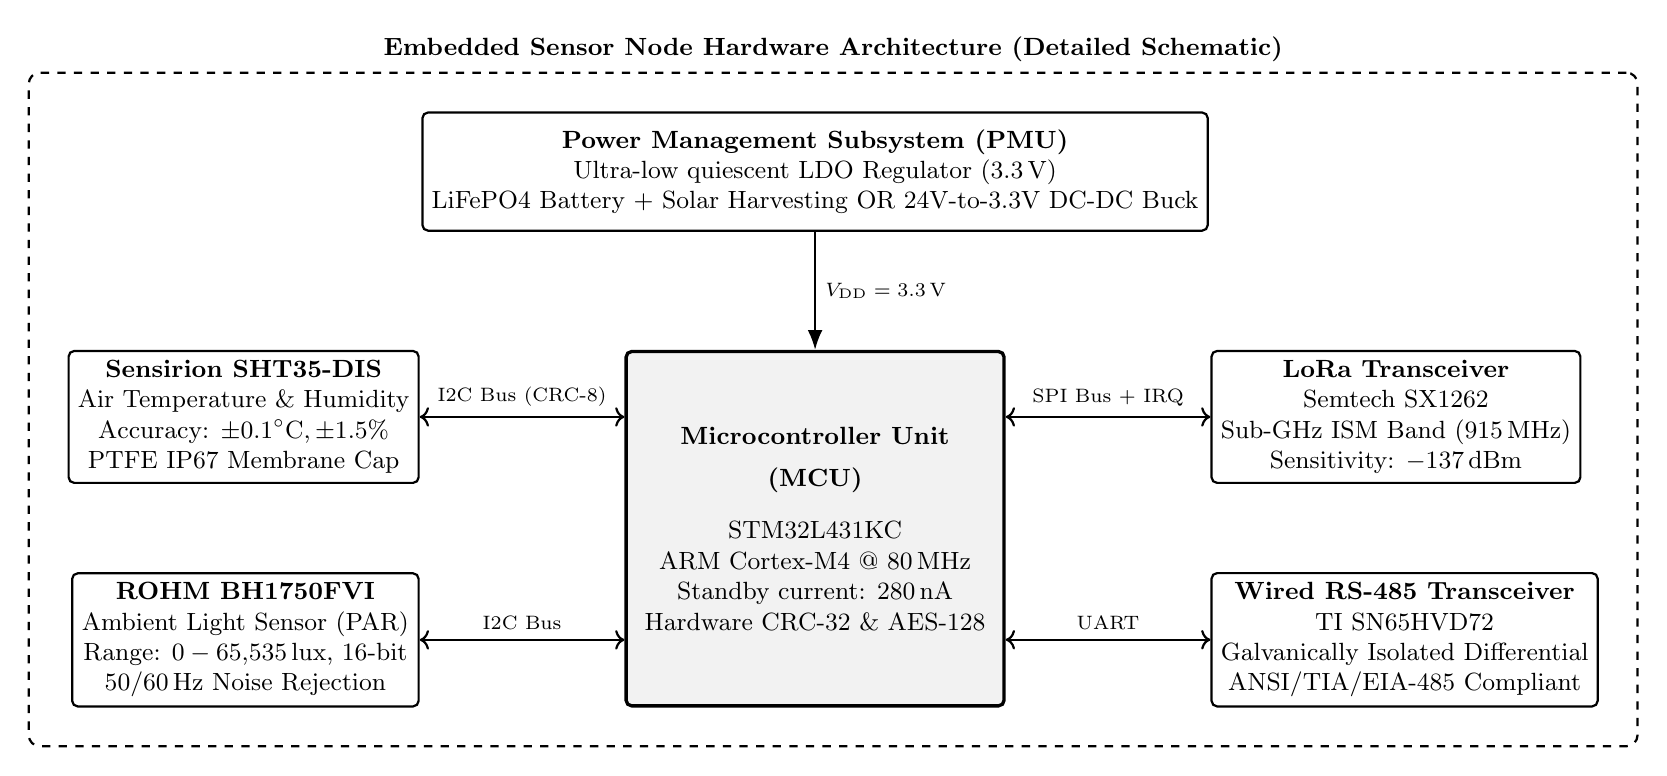
\begin{tikzpicture}[
    box/.style={rectangle, draw=black, fill=white, thick, rounded corners=2pt, minimum width=4.4cm, minimum height=1.5cm, align=center, font=\small},
    mcu/.style={rectangle, draw=black, fill=black!5, very thick, rounded corners=2pt, minimum width=4.8cm, minimum height=4.5cm, align=center, font=\small},
    line/.style={draw=black, thick, -{Latex[length=2.5mm]}}
]
    % Central MCU (Spacious & Clear)
    \node[mcu] (MCU) at (0,0) {
        \textbf{Microcontroller Unit}\\[4pt]
        \textbf{(MCU)}\\[8pt]
        STM32L431KC\\
        ARM Cortex-M4 @ 80\,MHz\\
        Standby current: $280\,\text{nA}$\\
        Hardware CRC-32 \& AES-128
    };
    
    % Left Sensors (Wide boxes for clear text)
    \node[box, left=2.6cm of MCU.north west, anchor=north east] (SHT) {
        \textbf{Sensirion SHT35-DIS}\\
        Air Temperature \& Humidity\\
        Accuracy: $\pm 0.1^\circ\text{C}, \pm 1.5\%$\\
        PTFE IP67 Membrane Cap
    };
    \node[box, left=2.6cm of MCU.south west, anchor=south east] (BH) {
        \textbf{ROHM BH1750FVI}\\
        Ambient Light Sensor (PAR)\\
        Range: $0 - 65{,}535\,\text{lux}$, 16-bit\\
        $50/60\,\text{Hz}$ Noise Rejection
    };
    
    % Right Communications (Wide boxes)
    \node[box, right=2.6cm of MCU.north east, anchor=north west] (TRANS1) {
        \textbf{LoRa Transceiver}\\
        Semtech SX1262\\
        Sub-GHz ISM Band ($915\,\text{MHz}$)\\
        Sensitivity: $-137\,\text{dBm}$
    };
    \node[box, right=2.6cm of MCU.south east, anchor=south west] (TRANS2) {
        \textbf{Wired RS-485 Transceiver}\\
        TI SN65HVD72\\
        Galvanically Isolated Differential\\
        ANSI/TIA/EIA-485 Compliant
    };
    
    % Top Power Management Subsystem
    \node[box, above=1.5cm of MCU, minimum width=7.2cm] (PWR) {
        \textbf{Power Management Subsystem (PMU)}\\
        Ultra-low quiescent LDO Regulator ($3.3\,\text{V}$)\\
        LiFePO4 Battery + Solar Harvesting OR 24V-to-3.3V DC-DC Buck
    };
    
    % Interconnections with clean bus annotations
    \draw[line, <->] (SHT) -- (MCU.north west |- SHT) node[midway, above, font=\scriptsize] {$\text{I2C Bus (CRC-8)}$};
    \draw[line, <->] (BH) -- (MCU.south west |- BH) node[midway, above, font=\scriptsize] {$\text{I2C Bus}$};
    \draw[line, <->] (MCU.north east |- TRANS1) -- (TRANS1) node[midway, above, font=\scriptsize] {SPI Bus + IRQ};
    \draw[line, <->] (MCU.south east |- TRANS2) -- (TRANS2) node[midway, above, font=\scriptsize] {UART};
    \draw[line] (PWR) -- (MCU) node[midway, right, font=\scriptsize] {$V_{\text{DD}} = 3.3\,\text{V}$};
    
    % Enclosing Frame - Draw.io style
    \begin{scope}[on background layer]
        \node[draw=black, dashed, thick, fill=white, rounded corners=4pt, fit=(SHT) (BH) (MCU) (TRANS1) (TRANS2) (PWR), inner sep=14pt, label={[font=\bfseries\small, text=black]above:Embedded Sensor Node Hardware Architecture (Detailed Schematic)}] {};
    \end{scope}
\end{tikzpicture}
}
\caption{Detailed hardware subsystem schematic of the multi-modal greenhouse sensor node.}
\label{fig:node_block_diagram}
\end{figure}

The selected sensor components offer industrial grade specifications:
\begin{itemize}
    \item \textbf{Sensirion SHT35-DIS:} Capacitive relative humidity sensor and band-gap temperature sensor housed behind a PTFE membrane filter cap (IP67). Supports wide operating voltages ($2.15\,\text{V} - 5.5\,\text{V}$) and embedded hardware alert pins.
    \item \textbf{ROHM BH1750FVI:} Calibrated ambient light sensor with built-in 16-bit ADC, human eye spectral response approximation, and rejection of $50/60\,\text{Hz}$ artificial light flicker.
    \item \textbf{Microcontroller (MCU):} STM32L431 (ARM Cortex-M4 running at $80\,\text{MHz}$), drawing only $280\,\text{nA}$ in standby mode with real-time clock (RTC) retention, providing native hardware CRC-32 and AES acceleration.
\end{itemize}

% =========================================================================
\section{Design 1: Low-Power Wireless Sensor Network (LoRaWAN)}
% =========================================================================

\subsection{Communication Infrastructure and Protocol Stack}
Design 1 deploys a star-of-stars wireless network based on the \textbf{LoRaWAN} Class A open standard operating in the license-free $915\,\text{MHz}$ ISM band (AS923 or US915 regional parameters) \cite{lora_alliance}.
\begin{itemize}
    \item \textbf{Modulation Physics:} LoRa utilizes Chirp Spread Spectrum (CSS) modulation, which trades transmission data rate for exceptional receiver sensitivity (down to $-137\,\text{dBm}$). Sub-GHz signals pass through moist foliage and greenhouse glass walls with significantly lower attenuation than $2.4\,\text{GHz}$ signals ($10-15\,\text{dB}$ lower path loss).
    \item \textbf{Modulation Parameters:} Spreading Factor $\text{SF}=7$, Bandwidth $\text{BW}=125\,\text{kHz}$, Coding Rate $\text{CR}=4/5$. The over-the-air time (Time-on-Air, ToA) for a $16$-byte payload is approximately $41\,\text{ms}$, well within the $1\%$ regional duty-cycle regulatory restriction.
    \item \textbf{Network Topology:} All ten sensor nodes broadcast directly to an 8-channel Industrial LoRaWAN Gateway mounted near the entrance at $X=0\,\text{m}$. The gateway relays encrypted uplink frames over Ethernet / 4G-LTE backhaul via MQTT to a central telemetry server.
\end{itemize}

\begin{figure}[H]
\centering
\resizebox{0.92\linewidth}{!}{
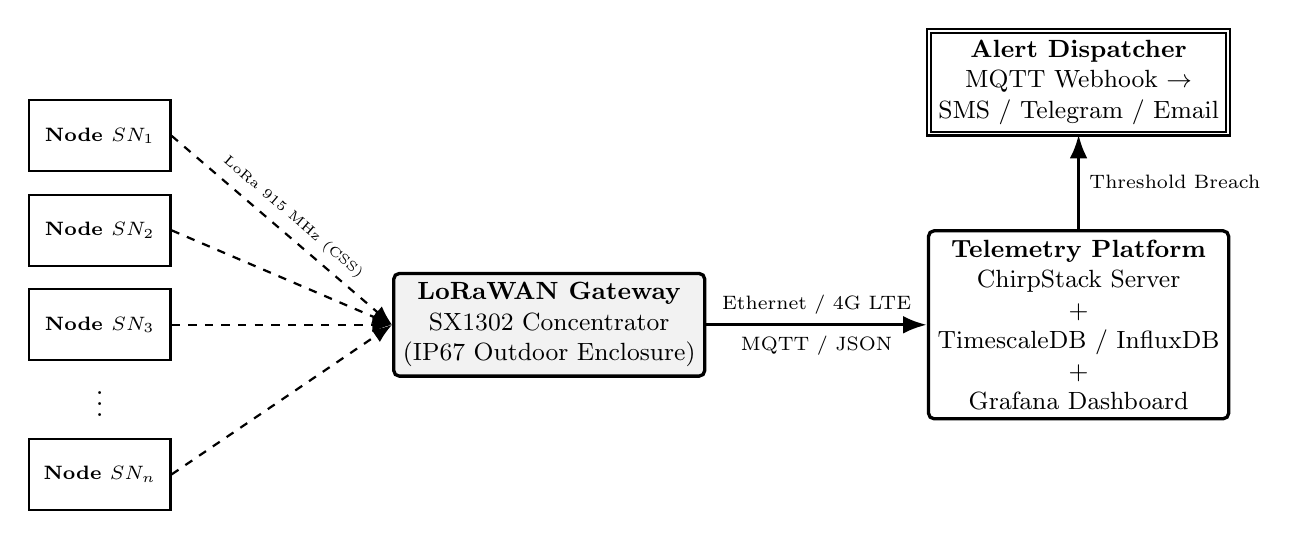
\begin{tikzpicture}[
    node distance=1.5cm and 2.0cm,
    node/.style={rectangle, draw=black, fill=white, thick, minimum width=1.8cm, minimum height=0.9cm, font=\bfseries\scriptsize, align=center},
    gw/.style={rectangle, draw=black, fill=black!5, very thick, rounded corners=2pt, minimum width=3.2cm, minimum height=1.3cm, align=center, font=\small},
    cloud/.style={rectangle, draw=black, fill=white, very thick, rounded corners=2pt, minimum width=3.4cm, minimum height=1.6cm, align=center, font=\small},
    alert/.style={rectangle, draw=black, double, fill=white, thick, minimum width=3.0cm, minimum height=1.1cm, align=center, font=\small},
    arr/.style={draw=black, thick, dashed, -{Latex[length=2.5mm]}},
    pipe/.style={draw=black, very thick, -{Latex[length=3mm]}}
]
    % Nodes
    \node[node] (N1) at (0, 2.4) {Node $SN_1$};
    \node[node] (N2) at (0, 1.2) {Node $SN_2$};
    \node[node] (N3) at (0, 0.0) {Node $SN_3$};
    \node[align=center, font=\normalsize] (Ndots) at (0, -0.9) {\vdots};
    \node[node] (N10) at (0, -1.9) {Node $SN_n$};
    
    % Gateway
    \node[gw, right=2.8cm of N3] (GW) {\textbf{LoRaWAN Gateway}\\SX1302 Concentrator\\(IP67 Outdoor Enclosure)};
    
    % Cloud / Edge Server
    \node[cloud, right=2.8cm of GW] (CLOUD) {\textbf{Telemetry Platform}\\ChirpStack Server\\+\\TimescaleDB / InfluxDB\\+\\Grafana Dashboard};
    
    % Alerting
    \node[alert, above=1.2cm of CLOUD] (NOTIF) {\textbf{Alert Dispatcher}\\MQTT Webhook $\to$\\SMS / Telegram / Email};
    
    % Connectors
    \draw[arr] (N1.east) -- node[above, sloped, font=\tiny] {LoRa 915 MHz (CSS)} (GW.west);
    \draw[arr] (N2.east) -- (GW.west);
    \draw[arr] (N3.east) -- (GW.west);
    \draw[arr] (N10.east) -- (GW.west);
    
    \draw[pipe] (GW) -- node[above, font=\scriptsize] {Ethernet / 4G LTE} node[below, font=\scriptsize] {MQTT / JSON} (CLOUD);
    \draw[pipe] (CLOUD) -- node[right, font=\scriptsize] {Threshold Breach} (NOTIF);
\end{tikzpicture}
}
\caption{System architecture for Design 1 (LoRaWAN Wireless Star Network).}
\label{fig:design1_arch}
\end{figure}

\subsection{Data Correctness Mechanisms}
In wireless environments, electromagnetic interference and frame collisions corrupt transmissions. Design 1 implements a multi-tier integrity framework:
\begin{enumerate}
    \item \textbf{Sensor Bus Checksum:} Communication between MCU and the SHT35 uses an 8-bit Cyclic Redundancy Check ($P(x) = x^8 + x^5 + x^4 + 1$ with initial value \texttt{0xFF}). Corrupted reads on the $\text{I}^2\text{C}$ bus are discarded locally.
    \item \textbf{MAC Layer Integrity:} The LoRa physical frame includes an embedded 16-bit CRC ($CRC-16$) calculated across the entire payload. Corrupted frames are dropped immediately at the gateway RF receiver.
    \item \textbf{Application Level Security and Integrity:} End-to-end payload encryption uses AES-128 in Cipher Block Chaining Message Authentication Code (CBC-MAC, RFC 4493), producing a 4-byte Message Integrity Code (MIC). This prevents packet spoofing or replay attacks.
    \item \textbf{Acknowledged Uplinks (ARQ):} In normal operation, sensor nodes send unconfirmed uplinks to minimize power consumption. If an anomalous parameter is detected (e.g., $T > 38^\circ\text{C}$), the node switches to \textit{Confirmed Uplink} mode with automatic retransmission (up to 3 retries with pseudo-random exponential backoff) until an explicit downstream ACK is received.
\end{enumerate}

\subsection{Power Budget and Battery Longevity Calculation}
Each wireless node is powered by an industrial $3.2\,\text{V}$, $3{,}000\,\text{mAh}$ Lithium Iron Phosphate ($\text{LiFePO}_4$) cell (chosen for thermal stability up to $60^\circ\text{C}$). The sampling cycle operates at $T_{\text{sample}} = 60\,\text{seconds}$:
\begin{itemize}
    \item \textbf{Active State (Wakeup, Sample Sensors, Compute CRC):} Duration $t_1 = 30\,\text{ms}$, average current $I_1 = 8\,\text{mA}$. Energy: $E_1 = 8\,\text{mA} \times 0.030\,\text{s} = 0.24\,\text{mA}\cdot\text{s}$.
    \item \textbf{Transmit State (LoRa TX at $+14\,\text{dBm}$):} Duration $t_2 = 41\,\text{ms}$, average current $I_2 = 45\,\text{mA}$. Energy: $E_2 = 45\,\text{mA} \times 0.041\,\text{s} = 1.845\,\text{mA}\cdot\text{s}$.
    \item \textbf{Receive Windows ($RX_1, RX_2$):} Duration $t_3 = 50\,\text{ms}$, average current $I_3 = 6\,\text{mA}$. Energy: $E_3 = 0.30\,\text{mA}\cdot\text{s}$.
    \item \textbf{Deep Sleep State ($59.88\,\text{s}$):} Current $I_{\text{sleep}} = 1.5\,\mu\text{A}$. Energy: $E_4 = 0.0015\,\text{mA} \times 59.88\,\text{s} \approx 0.09\,\text{mA}\cdot\text{s}$.
\end{itemize}
Total charge consumption per 60-second cycle:
\begin{equation}
Q_{\text{cycle}} = E_1 + E_2 + E_3 + E_4 = 0.24 + 1.845 + 0.30 + 0.09 = 2.475\,\text{mA}\cdot\text{s} = 0.0006875\,\text{mAh}
\end{equation}
Daily consumption: $Q_{\text{day}} = 0.0006875 \times 1440 = 0.99\,\text{mAh/day}$. With an 80\% usable battery capacity de-rating ($2{,}400\,\text{mAh}$), the theoretical battery operating life is:
\begin{equation}
\text{Battery Life} = \frac{2{,}400\,\text{mAh}}{0.99\,\text{mAh/day}} \approx 2{,}424\,\text{days} \approx 6.6\,\text{years}
\end{equation}
This confirms that battery replacement overhead is low during standard operation.

\subsection{Data Analysis Pipeline and Cloud Alerting}
Sensor telemetry collected at the gateway is routed to an IoT analytics platform (e.g., ThingsBoard or AWS IoT Core). The cloud system applies a rule engine to monitor micro-climate thresholds:
\begin{equation}
\text{Alert Condition} = \begin{cases}
    \textbf{Heat Stress Warning}, & \text{if } T > 35^\circ\text{C} \text{ for } \tau > 3\,\text{mins} \\
    \textbf{Fungal Risk (High VPD)}, & \text{if } RH > 90\% \text{ and } T \in [18^\circ\text{C}, 24^\circ\text{C}] \\
    \textbf{Insufficient Light (PAR)}, & \text{if } L < 5{,}000\,\text{lux between 08:00--16:00}
\end{cases}
\end{equation}
When an alert triggers, an automated notification pipeline dispatches actionable alerts via Webhook / Push / SMS to greenhouse operators.

% =========================================================================
\section{Design 2: Industrial Multi-Drop Wired Bus (RS-485 / Modbus RTU)}
% =========================================================================

\subsection{Communication Infrastructure and Bus Topology}
Design 2 deploys an industrial wired multi-drop bus conforming to the \textbf{TIA/EIA-485-A (RS-485)} standard operating with the \textbf{Modbus RTU} protocol \cite{modbus_org}.
\begin{itemize}
    \item \textbf{Physical Layer Signaling:} RS-485 uses balanced differential signaling across a twisted-wire pair ($A$ and $B$). The receiver senses the differential voltage $V_{AB} = V_A - V_B$. Common-mode noise generated by high-power irrigation pumps and ventilation inverters couples equally into both conductors and is eliminated by the receiver's high Common-Mode Rejection Ratio (CMRR $> 70\,\text{dB}$).
    \item \textbf{Cabling and Power-over-Bus:} A cable is routed along the central walkway of the $50$\,m greenhouse:
    \begin{itemize}
        \item Pair 1 (Shielded Twisted): Modbus Data lines ($A$ and $B$).
        \item Pair 2 (Heavy Gauge): Centralized $24\,\text{VDC}$ power supply ($V_{\text{BUS}+}$ and $GND$).
    \end{itemize}
    Each sensor node integrates a high-efficiency DC-DC step-down buck converter (e.g., TI LM5164) that steps down $24\,\text{VDC}$ to $3.3\,\text{VDC}$ locally, avoiding significant $I^2R$ voltage drop across the $50$\,m run.
    \item \textbf{Bus Termination and Topology:} Pure linear daisy-chain topology without stubs (stubs $< 10\,\text{cm}$). Both cable ends are terminated with $120\,\Omega$ metal-film resistors matching the characteristic impedance of the transmission line ($Z_0 = 120\,\Omega$), eliminating signal reflections.
\end{itemize}

\begin{figure}[H]
\centering
\resizebox{\linewidth}{!}{
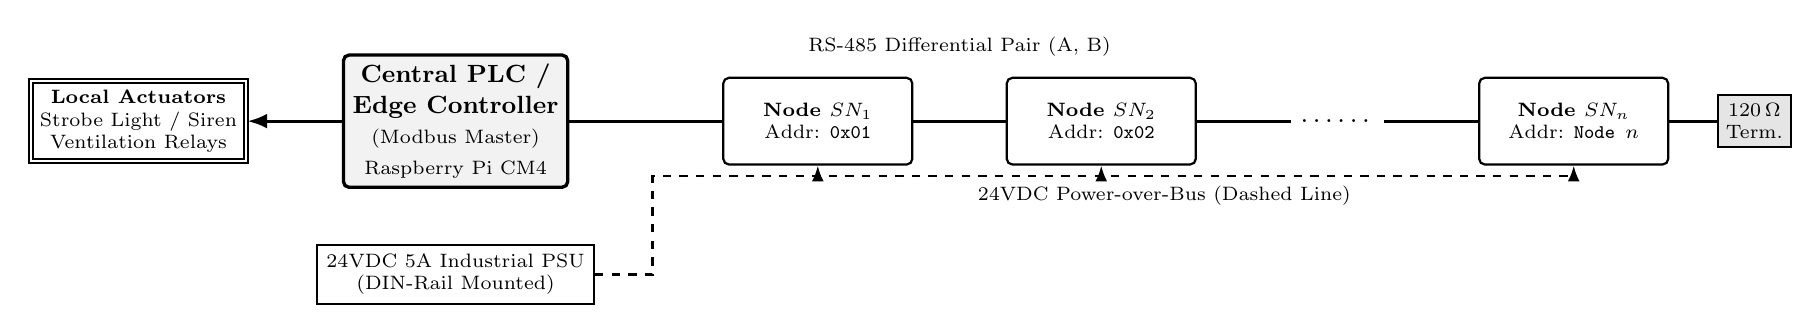
\begin{tikzpicture}[
    master/.style={rectangle, draw=black, fill=black!5, very thick, rounded corners=2pt, minimum width=2.8cm, minimum height=1.3cm, align=center, font=\small},
    nodebox/.style={rectangle, draw=black, fill=white, thick, rounded corners=2pt, minimum width=2.4cm, minimum height=1.1cm, align=center, font=\scriptsize},
    busline/.style={draw=black, very thick},
    pwrline/.style={draw=black, thick, dashed},
    drop/.style={draw=black, thick, -{Latex[length=2mm]}}
]
    % Central Controller Master
    \node[master] (MASTER) at (-1, 0) {\textbf{Central PLC /}\\\textbf{Edge Controller}\\\scriptsize(Modbus Master)\\\scriptsize Raspberry Pi CM4};
    
    % Industrial Power Supply
    \node[rectangle, draw=black, fill=white, thick, below=0.7cm of MASTER, minimum width=2.8cm, align=center, font=\scriptsize] (PSU) {24VDC 5A Industrial PSU\\(DIN-Rail Mounted)};
    
    % Sensor Nodes in Daisy Chain with SN_n notation
    \node[nodebox] (SN1) at (3.6, 0) {\textbf{Node $SN_1$}\\Addr: \texttt{0x01}};
    \node[nodebox] (SN2) at (7.2, 0) {\textbf{Node $SN_2$}\\Addr: \texttt{0x02}};
    
    % Ellipsis representation
    \node[align=center, font=\normalsize] (DOTS) at (10.2, 0) {\dots\dots};
    
    \node[nodebox] (SNN) at (13.2, 0) {\textbf{Node $SN_n$}\\Addr: \texttt{Node $n$}};
    
    % Termination resistor
    \node[draw=black, fill=black!10, thick, inner sep=3pt, right=0.6cm of SNN, align=center, font=\scriptsize] (TERM) {$120\,\Omega$\\Term.};
    
    % Bus wires
    \draw[busline] (MASTER.east) -- (SN1.west);
    \draw[busline] (SN1.east) -- (SN2.west);
    \draw[busline] (SN2.east) -- (DOTS.west);
    \draw[busline] (DOTS.east) -- (SNN.west);
    \draw[busline] (SNN.east) -- (TERM.west);
    
    \node[above, font=\scriptsize] at (5.4, 0.7) {RS-485 Differential Pair (A, B)};
    
    % Power wires
    \draw[pwrline] (PSU.east) -| (1.5, -0.7) -- (13.2, -0.7);
    \draw[drop] (3.6, -0.7) -- (SN1.south);
    \draw[drop] (7.2, -0.7) -- (SN2.south);
    \draw[drop] (13.2, -0.7) -- (SNN.south);
    \node[below, font=\scriptsize] at (8.0, -0.7) {24VDC Power-over-Bus (Dashed Line)};
    
    % Alert outputs from Master
    \node[rectangle, draw=black, double, fill=white, thick, left=1.2cm of MASTER, minimum height=1.0cm, align=center, font=\scriptsize] (ALARM) {\textbf{Local Actuators}\\Strobe Light / Siren\\Ventilation Relays};
    \draw[draw=black, very thick, -{Latex[length=2.5mm]}] (MASTER.west) -- (ALARM.east);
\end{tikzpicture}
}
\caption{System architecture for Design 2 (Wired Daisy-Chain RS-485 / Modbus RTU Bus with $SN_n$ node scaling).}
\label{fig:design2_arch}
\end{figure}

\subsection{Modbus RTU Polling and Data Correctness}
Modbus RTU operates on a strict Master-Slave polling model. The Central Controller is the Master, and nodes $N_1 - N_{10}$ are Slaves with unique hardware addresses ($\texttt{0x01}$ to $\texttt{0x0A}$):
\begin{enumerate}
    \item \textbf{Deterministic Polling Schedule:} The Master polls each slave sequentially at a baud rate of $19{,}200\,\text{bps}$ (8-N-1 format). The Master transmits a 8-byte \texttt{Read Holding Registers (0x03)} request.
    \item \textbf{Error Detection with CRC-16-IBM:} The 16-bit CRC polynomial $G(x) = x^{16} + x^{15} + x^2 + 1$ is calculated across all bytes. If the computed CRC does not match at the Master, the packet is rejected and retried up to three times.
    \item \textbf{Bus Timing Determinism:} At $19{,}200\,\text{bps}$, reading 6 registers (12 bytes) takes approximately $15\,\text{ms}$ per slave node. Polling all 10 nodes completes in under $200\,\text{ms}$, providing real-time deterministic updates suitable for closed-loop environmental control.
\end{enumerate}

\subsection{Edge Computing and Autonomous Alert Architecture}
Unlike cloud-dependent systems, Design 2 performs all data analysis and anomaly detection \textbf{on the Edge} inside the Central Industrial Controller:
\begin{itemize}
    \item \textbf{Zero Cloud Dependency:} The system maintains complete alerting and fail-safe automation even during an external Internet or cellular outage.
    \item \textbf{Hardwired Relay Outputs:} The controller directly drives 230VAC contactor relays via opto-isolated outputs, enabling automated physical mitigation:
    \begin{itemize}
        \item If $T > 36^\circ\text{C}:$ Immediately energize roof ventilation motors and evaporative cooling pads.
        \item If $RH > 92\% :$ Engage forced de-humidification exhaust fans.
        \item If any node fails to respond for 3 consecutive poll cycles: Trigger an acoustic fault alarm (broken wire or transceiver failure).
    \end{itemize}
\end{itemize}

% =========================================================================
\section{Data Correctness and Anomaly Detection Workflow}
% =========================================================================

Regardless of the underlying physical communication medium, the raw measurements from the greenhouse environment must pass through a data cleaning and validation pipeline to prevent false alarms caused by electrical noise, condensation drops on sensor elements, or momentary shadowing.

\begin{figure}[H]
\centering
\resizebox{0.78\linewidth}{!}{
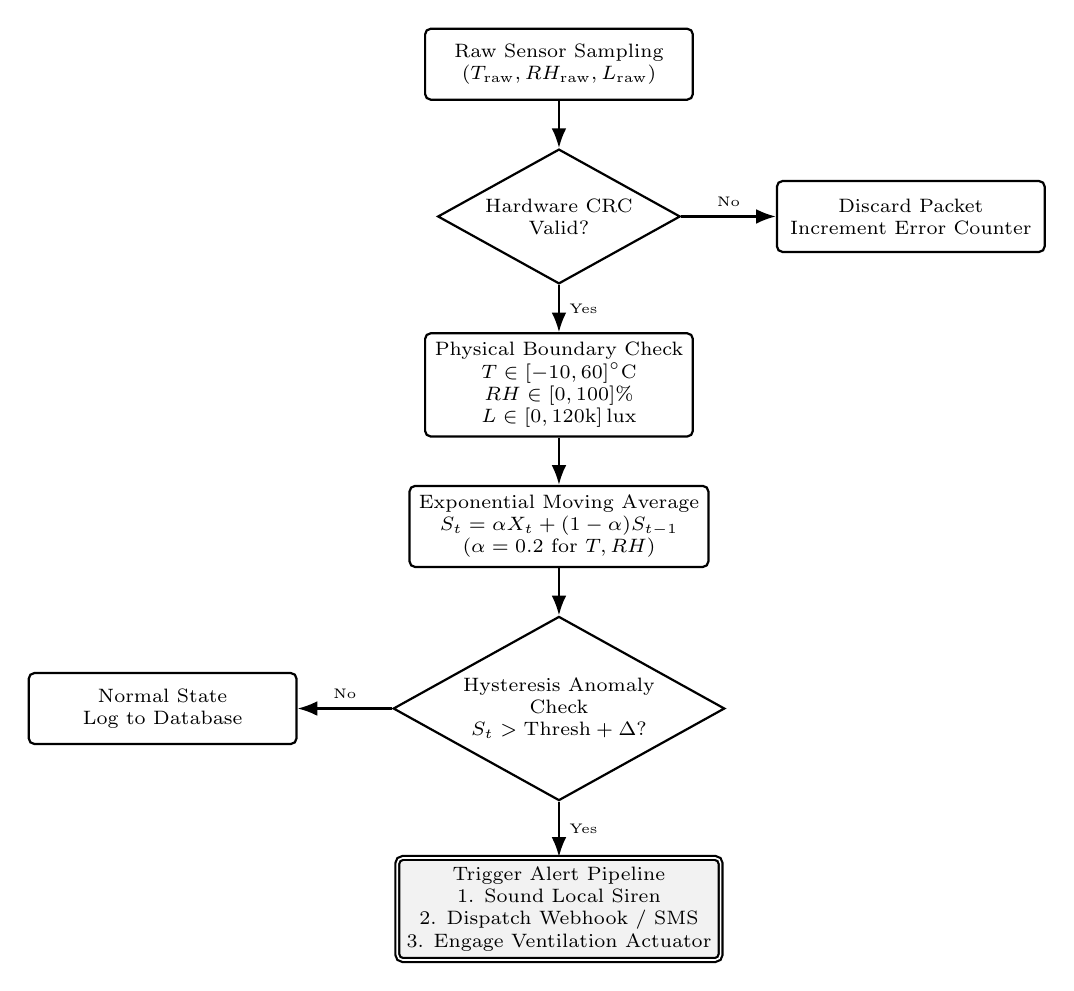
\begin{tikzpicture}[
    block/.style={rectangle, draw=black, fill=white, thick, rounded corners=2pt, minimum width=3.4cm, minimum height=0.9cm, align=center, font=\scriptsize},
    decision/.style={diamond, draw=black, fill=white, thick, aspect=1.8, inner sep=2pt, align=center, font=\scriptsize},
    alertbox/.style={rectangle, draw=black, double, fill=black!5, thick, rounded corners=2pt, minimum width=3.0cm, minimum height=0.9cm, align=center, font=\scriptsize},
    line/.style={draw=black, thick, -{Latex[length=2.5mm]}}
]
    \node[block] (raw) {Raw Sensor Sampling\\($T_{\text{raw}}, RH_{\text{raw}}, L_{\text{raw}}$)};
    \node[decision, below=0.6cm of raw] (chksum) {Hardware CRC\\Valid?};
    \node[block, right=1.2cm of chksum] (discard) {Discard Packet\\Increment Error Counter};
    
    \node[block, below=0.6cm of chksum] (phys) {Physical Boundary Check\\$T \in [-10, 60]^\circ\text{C}$\\$RH \in [0, 100]\%$\\$L \in [0, 120\text{k}]\,\text{lux}$};
    
    \node[block, below=0.6cm of phys] (filter) {Exponential Moving Average\\$S_t = \alpha X_t + (1-\alpha)S_{t-1}$\\($\alpha = 0.2$ for $T, RH$)};
    
    \node[decision, below=0.6cm of filter] (thresh) {Hysteresis Anomaly\\Check\\$S_t > \text{Thresh} + \Delta$?};
    
    \node[block, left=1.2cm of thresh] (normal) {Normal State\\Log to Database};
    \node[alertbox, below=0.7cm of thresh] (alert) {Trigger Alert Pipeline\\1. Sound Local Siren\\2. Dispatch Webhook / SMS\\3. Engage Ventilation Actuator};

    % Connections
    \draw[line] (raw) -- (chksum);
    \draw[line] (chksum) -- node[above, font=\tiny] {No} (discard);
    \draw[line] (chksum) -- node[right, font=\tiny] {Yes} (phys);
    \draw[line] (phys) -- (filter);
    \draw[line] (filter) -- (thresh);
    \draw[line] (thresh) -- node[above, font=\tiny] {No} (normal);
    \draw[line] (thresh) -- node[right, font=\tiny] {Yes} (alert);
\end{tikzpicture}
}
\caption{Data validation, digital noise filtering, and hysteresis-based alert workflow (Draw.io monochrome style).}
\label{fig:alert_flowchart}
\end{figure}

\subsection{Digital Filtering and Outlier Rejection}
To smooth out transient measurement spikes (e.g., brief direct sunbeam hitting a sensor or sudden mist droplet), an Exponential Moving Average filter runs over the validated stream:
\begin{equation}
S_t = \alpha \cdot X_t + (1 - \alpha) \cdot S_{t-1}
\end{equation}
where $X_t$ is the current raw validated reading, $S_t$ is the smoothed state, and $\alpha = 0.2$ is the smoothing factor. For rapid transient spikes (e.g., $|\Delta X_t / \Delta t| > 5^\circ\text{C/min}$), readings are flagged as transient artifacts and require 3 consecutive corroborating samples before updating the internal alert state.

\subsection{Hysteresis Thresholding for Alert Stability}
To prevent alert oscillation around threshold boundaries (chattering), the system enforces deadband hysteresis:
\begin{equation}
\text{Alarm Status} = \begin{cases}
    \textbf{ACTIVE}, & \text{if } T_{\text{filt}} \ge T_{\text{high}} \quad (35.0^\circ\text{C}) \\
    \textbf{CLEAR},  & \text{if } T_{\text{filt}} \le T_{\text{high}} - T_{\text{hyst}} \quad (33.0^\circ\text{C}) \\
    \textbf{HOLD},   & \text{if } 33.0^\circ\text{C} < T_{\text{filt}} < 35.0^\circ\text{C}
\end{cases}
\end{equation}

% =========================================================================
\section{Comprehensive Trade-Off Analysis}
% =========================================================================

Table~\ref{tab:detailed_tradeoff} summarizes the core engineering trade-offs between Design~1 (LoRaWAN Wireless) and Design~2 (RS-485 Wired), with each architectural characteristic substantiated by published standards and peer-reviewed literature.

\begin{table}[H]
\centering
\small
\renewcommand{\arraystretch}{1.3}
\begin{tabularx}{\textwidth}{>{\bfseries}p{2.7cm} X X >{\centering\arraybackslash}p{2.2cm}}
\toprule
Trade-Off Dimension & Design 1: Wireless (LoRaWAN) & Design 2: Wired (RS-485 / Modbus) & Verified Ref. \\
\midrule
1. Communication Infrastructure & 
Zero cabling; rapid deployment; nodes can be relocated dynamically to follow crop rotations. & 
Fixed daisy-chain topology; requires shielded twisted-pair conduits and $120\,\Omega$ termination. & 
\cite{lora_alliance, rs485_standard} \\

2. Data Correctness \& Reliability & 
RF path loss due to foliage absorption and metal frames; mitigated via CRC-16 and ARQ retries. & 
Differential signaling with high common-mode rejection (CMRR $>70\,\text{dB}$); immune to motor/inverter EMI. & 
\cite{rs485_standard, greenhouse_microclimate} \\

3. Alert Latency \& Determinism & 
Non-deterministic random access (Aloha); delivery latency $1 - 5$\,s; cloud-dependent alerting pipeline. & 
Deterministic cyclic polling ($<200$\,ms for 10 nodes); sub-second local Edge actuator/siren triggering. & 
\cite{modbus_org, modbus_agriculture} \\

4. Power Supply \& Maintenance & 
Autonomous battery-powered ($\text{LiFePO}_4$ life $\approx 6.6$\,years); requires periodic battery inspection. & 
Continuous centralized 24\,VDC Power-over-Bus; zero battery maintenance; single central UPS backup. & 
\cite{iot_agri, modbus_agriculture} \\

5. Cost Profile (CAPEX vs. OPEX) & 
Low initial installation cost ($\approx \$600$); higher per-node transceiver silicon cost. & 
Higher initial installation cost ($\approx \$1{,}200$ for cabling/conduits); lower per-node silicon cost. & 
\cite{wsn_review, modbus_agriculture} \\
\bottomrule
\end{tabularx}
\caption{Streamlined engineering trade-off comparison between Wireless and Wired designs with literature verification.}
\label{tab:detailed_tradeoff}
\end{table}

\subsection{Engineering Selection and Deployment Guidelines}
\begin{itemize}
    \item \textbf{Select Design 1 (Wireless LoRaWAN) when:}
    \begin{itemize}
        \item The greenhouse utilizes modular hydroponic benches or seasonal crop rotations where spatial reconfiguration occurs frequently.
        \item The facility is an existing structure where retrofitting conduits is cost-prohibitive.
        \item Low-frequency telemetry ($1-5$\,minute intervals) is sufficient for operational monitoring.
    \end{itemize}
    \item \textbf{Select Design 2 (Wired RS-485 / Modbus) when:}
    \begin{itemize}
        \item The monitoring system directly controls critical automated actuators (emergency vents, heating valves, misting pumps) requiring sub-second deterministic response.
        \item The greenhouse operates heavy industrial inverters, large inductive fans, and high-frequency artificial lighting producing severe EMI.
        \item Long-term permanent installation with minimum maintenance is prioritized over initial setup cost.
    \end{itemize}
\end{itemize}

% =========================================================================
\section{Conclusion}
% =========================================================================
This report proposed two end-to-end embedded system architectures for micro-climate monitoring in a $20 \times 50$\,m greenhouse facility, addressing communication infrastructure, data correctness, and automated alerting. Design 1 utilizes a Sub-GHz LoRaWAN wireless star topology, providing a calculated battery lifetime exceeding 6 years and maximum spatial flexibility. Design 2 deploys an industrial differential RS-485 Modbus RTU wired bus, ensuring deterministic sub-200\,ms cycle times, complete EMI immunity, and fully autonomous edge-based alarm processing. Both designs incorporate multi-tier data correctness techniques, including hardware CRCs, physical boundary filtering, exponential smoothing, and hysteresis-bounded alert escalation.

% =========================================================================
% REFERENCES
% =========================================================================
\begin{thebibliography}{99}

\bibitem{sht35_datasheet}
Sensirion AG, 
\textit{Datasheet SHT3x-DIS: Humidity and Temperature Sensor IC}, 
Version 7, Dec. 2019. [Online]. Available: \url{https://www.sensirion.com}

\bibitem{lora_alliance}
LoRa Alliance, 
\textit{LoRaWAN 1.0.4 Regional Parameters Specification}, 
LoRa Alliance Technical Committee, Oct. 2020.

\bibitem{modbus_org}
Modbus Organization, 
\textit{Modbus Application Protocol Specification V1.1b3}, 
Dec. 2012. [Online]. Available: \url{http://www.modbus.org}

\bibitem{rs485_standard}
Telecommunications Industry Association (TIA), 
\textit{Electrical Characteristics of Generators and Receivers for Use in Balanced Digital Multipoint Systems (ANSI/TIA/EIA-485-A-98)}, 
Reaffirmed 2003.

\bibitem{iot_agri} 
O. Elijah, T. A. Rahman, I. Orikumhi, C. Y. Leow, and M. N. Hindia, 
``An Overview of Internet of Things (IoT) and Data Analytics in Agriculture: Benefits and Challenges,'' 
\textit{IEEE Internet of Things Journal}, vol. 5, no. 5, pp. 3758--3773, Oct. 2018.

\bibitem{wsn_review} 
T. Ojha, S. Misra, and N. S. Raghuwanshi, 
``Wireless Sensor Networks for Agriculture: The State-of-the-Art in Practice and Future Challenges,'' 
\textit{Computers and Electronics in Agriculture}, vol. 118, pp. 66--84, Oct. 2015.

\bibitem{greenhouse_microclimate}
L. Shamshiri et al., 
``Advances in greenhouse automation and controlled environment agriculture: A review of scientific research,'' 
\textit{International Journal of Agricultural and Biological Engineering}, vol. 11, no. 1, pp. 21--35, Jan. 2018.

\bibitem{modbus_agriculture}
R. G. Lins and P. R. M. de Oliveira, 
``Development of an industrial automation system for greenhouse monitoring using Modbus protocol,'' 
\textit{Computers and Electronics in Agriculture}, vol. 162, pp. 789--798, Jul. 2019.

\end{thebibliography}

\end{document}
